\section{Ergebnisse}
\subsection{Physische Risiko}
Die Hochwasserrisikostufen im erstellten Portfolio sind wie folgt verteilt: 1 hohes, 17 mittlere, 12 niedrige und 3823 sehr niedrige Risiken. Diese Risikostufeverteilung wird in Abbildung \ref{fig:riskostufe} graphisch dargestellt und visualisiert.
\begin{figure}[htbp]
    \centering
    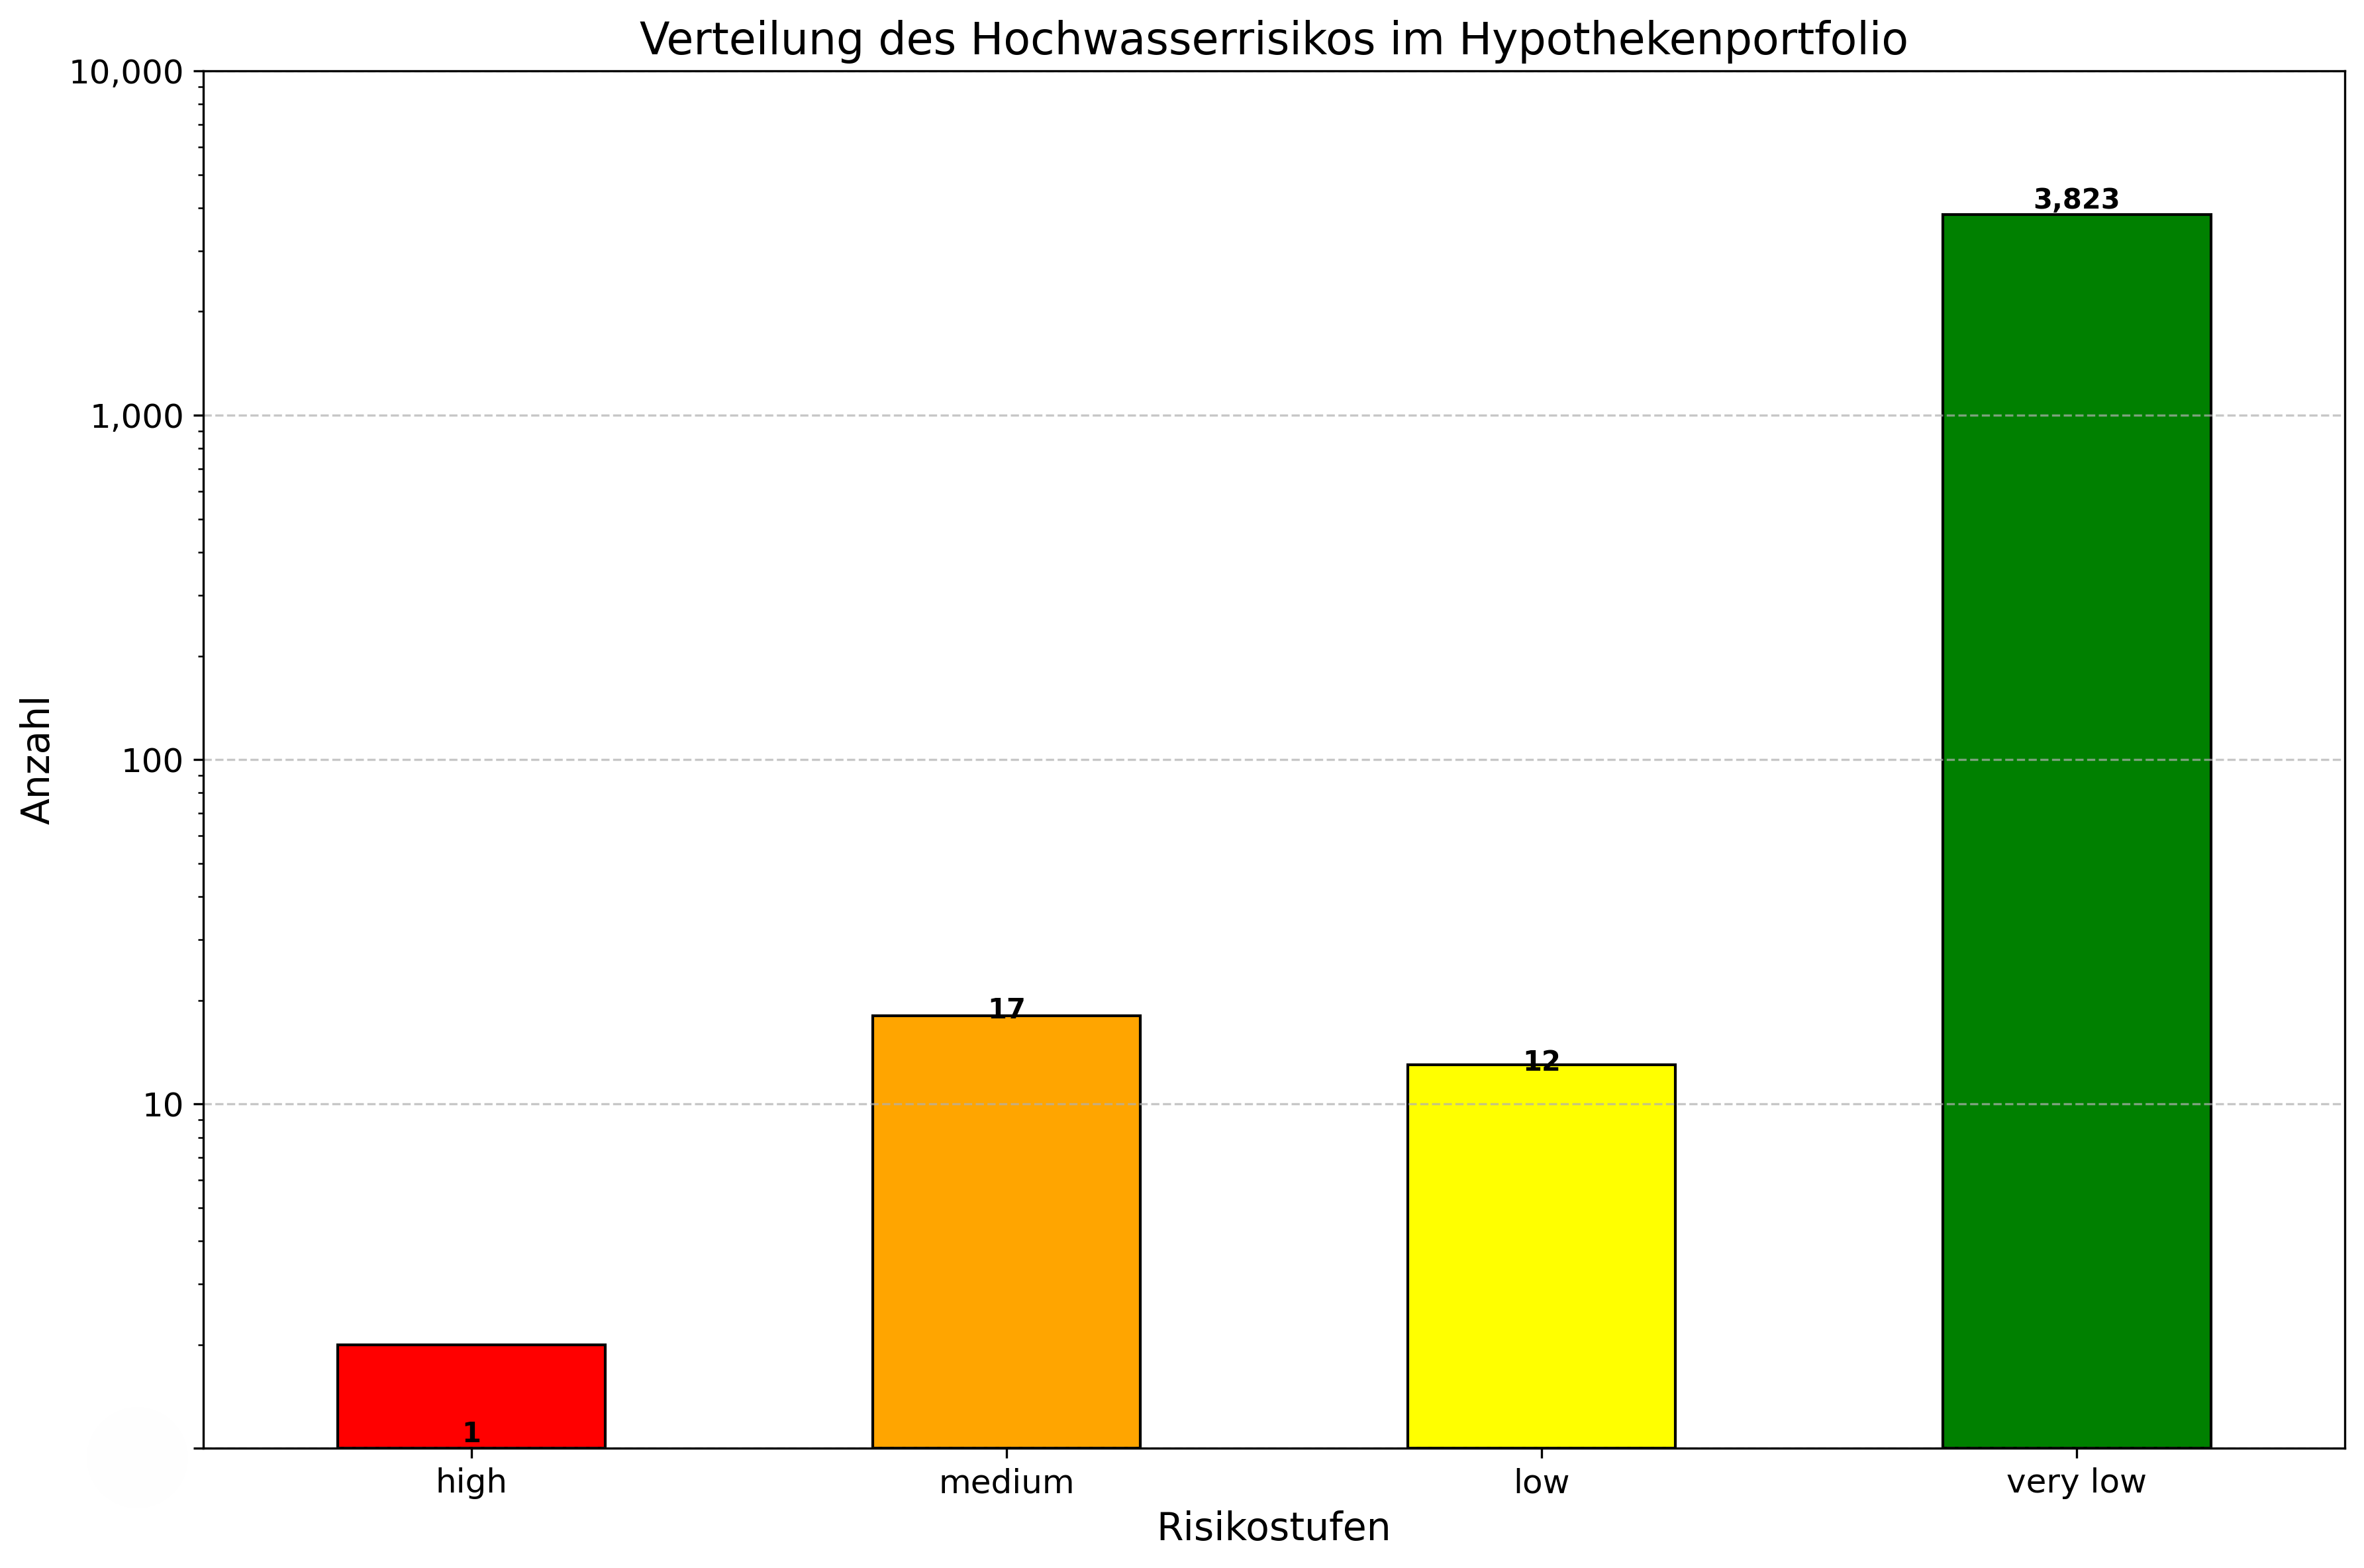
\includegraphics[width=\textwidth]{figures/hochwasserrisiko_verteilung.png}
    \caption{Verteilung der Hochwasserrisikostufen im Hypothekenportfolio. Quelle: Eigene Darstellung}
    \label{fig:riskostufe}
\end{figure}
\FloatBarrier
Mittels des digitalen Geländemodells von Bayerns sowie Pegelnullpunkt und Hochwasserstand von \textcite{bayern2016hochwassernachrichtendienst} wurde die Überflutungstiefe bestimmt. Dies betrifft Datenpunkte in den Kategorien hoch, mittel und niedrig.
Aufgrund der Größe der \ac{DGM}-Daten (240 GB) erfolgte die Berechnung nur für 30 Punkte in Hochrisiko-, mittlerem und niedrigem Risikogebiet. Entsprechende Orts-, Gemeinde- und Landkreisdaten wurden geladen.
Im Hochrisikogebiet liegt ein einzelner Punkt in Haag an der Amper. Dort beträgt die maximale Überflutungstiefe 2,1 m, entsprechend einem Schadensfaktor von 0,16.
17 Datenpunkte befinden sich in Gebieten mittleren Risikos, verteilt auf verschiedene Orte.In der Kategorie mittleres Risiko gibt es Punkte mit einer Überschwemmungstiefe von 0. Dies ist durchaus plausibel. Innerhalb eines Gebiets mit mittlerem Risiko variiert die Topographie. Höher gelegene Standorte weisen eine geringere Überflutungstiefe auf. Ähnlich verhält es sich mit 12 Datenpunkten in Gebieten mit niedrigem Risiko. Auch dort können nicht-null Überschwemmungstiefen auftreten. Dies ist auf die niedrigere Geländehöhe zurückzuführen. 

Die Ermittlung der Tiefe für 3823 Datenpunkte in sehr niedrigen Risikogebieten wurde nicht durchgeführt. Diese Datenpunkte umfassen 1518 Orte, verteilt über 72 Landkreise. Eine individuelle Bewertung ist sehr aufwendig, da alle Kartendaten manuell geladen werden müssen und kein vollständiger Datensatz für Bayern mit Pegelnullpunkten und Hochwasserständen vorhanden ist. Diese Informationen müssen zudem auch manuell gesucht werden. Aufgrund dieser Einschränkungen wurden für alle Datenpunkte in sehr niedrigen Risikogebieten eine Überflutungstiefe und Schadensfaktor von 0 angenommen.

Nach der Berechnung der Überflutungstiefe kann durch den Vergleich mit der Schadenfunktion in Abbildung \ref{fig:damage_curve2} der entsprechende Schadensfaktor ermittelt werden. Basierend auf diesem Schadensfaktor lässt sich mithilfe der Gleichung \ref{eq:schaden} der Immobilienschaden quantifizieren. Die Resultate dieser Berechnungen für den Immobilienschaden werden anschließend in Abbildung \ref{fig:schadenwert} grafisch dargestellt.
\begin{figure}[htbp]
    \centering
    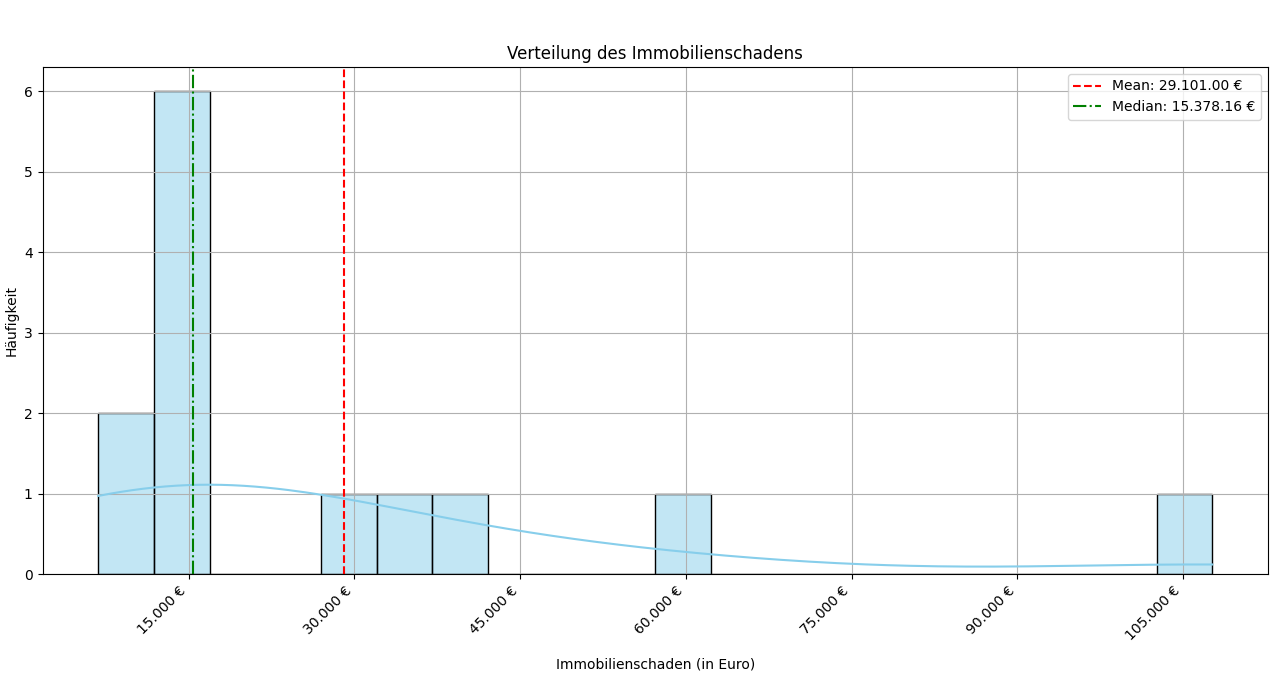
\includegraphics[width=\textwidth]{figures/flutschaden.png}
    \caption{Verteilung des Immobilienschaden im Hypothekenportfolio. Quelle: Eigene Darstellung}
    \label{fig:schadenwert}
\end{figure}
\FloatBarrier
Abbildung \ref{fig:schadenwert} zeigt eine rechtsschiefe Verteilung des Immobilienschadens, wobei die Mehrheit der Fälle im Bereich von etwa 8.000 bis 20.000 liegt. Der Median von 23.275,68 € liegt signifikant unter dem arithmetischen Durchschnitt von 35.558,03 €, was darauf hindeutet, dass es eine Ausreißer mit sehr hohen Schadensbeträgen gibt.